\section{ARP4761: Wheel Brake System}

%\mike{Move the generic description to a section right after the ``safety'' section along with the ARP figure.  Leave the modeling that we did in AADL here.  That way we can reference it in the MBSA sections.}
%\danielle{The whole nominal model description is here. The modeling we did is in the faults section.}

As a preliminary case study, we utilized the Wheel Brake System described in ARP 4761 - Appendix L \cite{AIR6110}. The Wheel Brake System is installed on the two main landing gears and is used during taxi, landing, and rejected take off. Braking is either commanded manually using brake pedals or automatically with no need for the pedals (autobrake). When the wheels have traction, the autobrake function will provide a constant smooth deceleration.

%%%%%%%%%%%% Try to get a better figure here... this one is all blurry...
\begin{figure}
\begin{center}
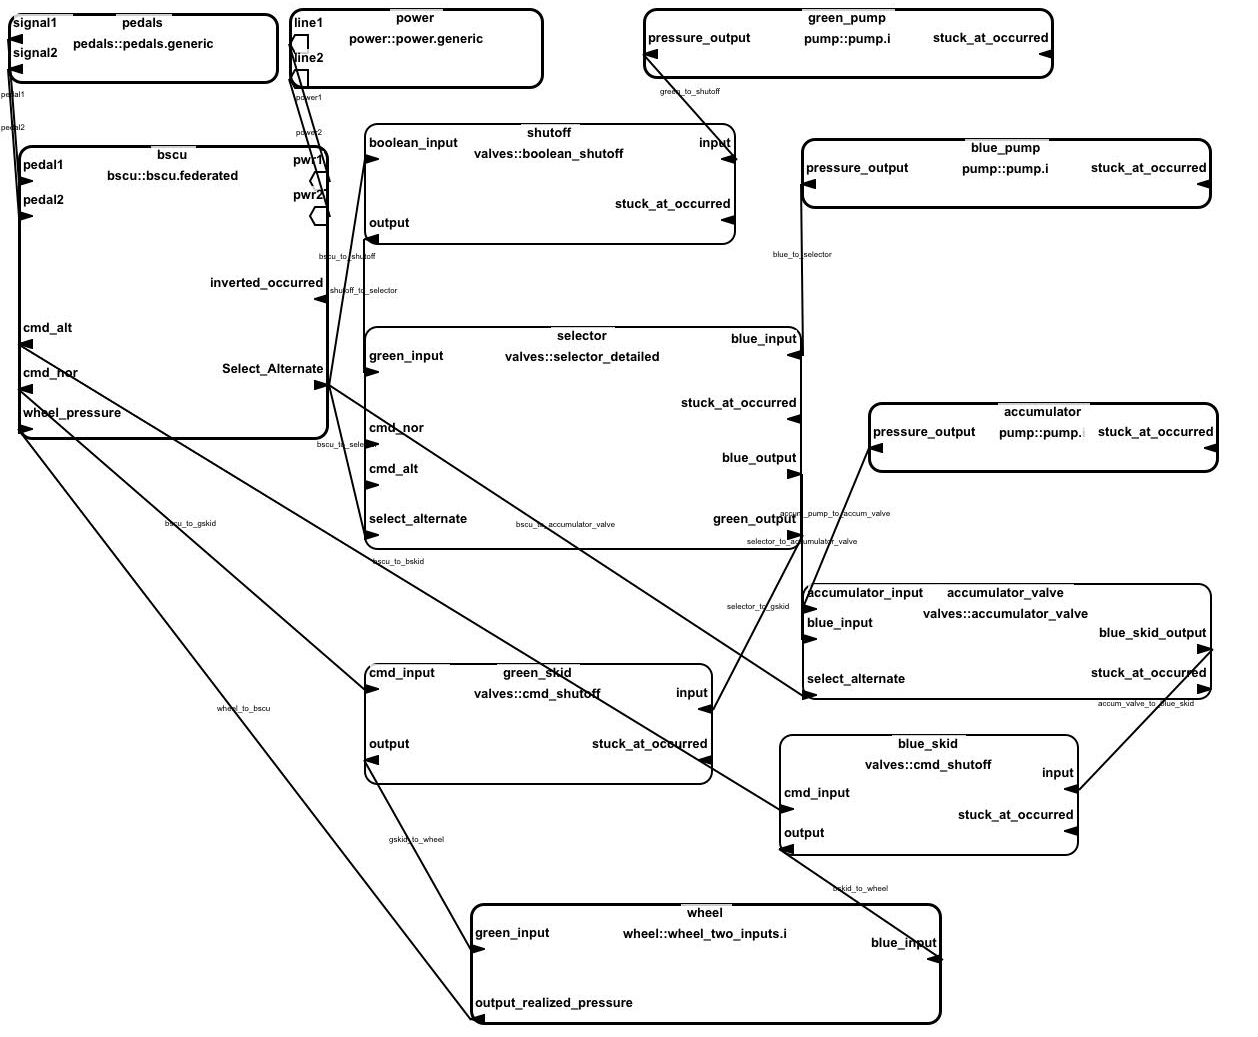
\includegraphics[scale=.37]{images/wbsfederated2.jpg}
\caption{AADL Simple Model of the Wheel Brake System }\label{fig:wbs_ima}
\mike{NOTE: selector::select\_alternate is not connected (we fixed this in our model)}
\mike{maybe we could add the modified portion of the model into the figure}
\danielle{The connection is added.}
\end{center}
\end{figure}

Each wheel has a brake assembly that is operated by two sets of hydraulic pistons which operate independently. One set is operated by the Green hydraulic line which is used in Normal braking mode. The second system (Alternate) is operated by the Blue hydraulic line which is used when the Normal system fails. The Alternate system is also supplied by an Accumulator which is a device with built up pressure that can be released if both of the two primary pumps (Blue and Green) fail. The accumulator supplies the Alternate system in case of Emergency braking mode.

Switching between the hydraulic pistons and sources can be done automatically or manually. If the Normal pressure (Green) is below a certain threshold, there is an automatic switchover to the Blue supply. If the Blue pump fails, then the Accumulator is used for hydraulic pressure.

In both Normal and Alternate modes, an anti-skid capability is available. In the Normal mode, the brake pedal position is electronically fed to a braking computer called the Braking System Control Unit (BSCU). The BSCU monitors signals that denote critical aircraft and system states to provide correct braking function, detect anomalies, broadcast warnings, and sent maintenance information to other systems.

\subsection{Nominal System Modeling}
A formal specification of the nominal system model consists of mechanical and digital components and their interconnections. Figure~\ref{fig:wbs_ima} illustrates how the wheel braking system is modeled using Architecture Analysis and Design Language (AADL). The following section describes this nominal model from which the fault model was generated.

\paragraph{Wheel Braking System (WBS)}
The highest level component is the WBS. It consists of a digital control unit, the BSCU, and Normal and Alternate hydraulic pressure lines (supplied by Green Pump and Blue Pump/Accumulator respectively), a Selector which selects between Normal and Alternate modes of hydraulic pressure, and the Wheel system. The WBS takes inputs from the environment including PedalPos1, AutoBrake, DecRate, AC\_Speed, and Skid. All of these inputs are forwarded to the BSCU to compute the brake commands.

\paragraph{Braking System Control Unit (BSCU)}
The BSCU is the digital component in the system that receives inputs from the WBS. It also receives feedback from the Normal and Alternate lines and two power inputs from two separate power sources. The BSCU is composed of two Command and Monitor subsystems each powered independently from separate power sources. The pedal position maps into these units and when skidding occurs, the Command and Monitor units will decrease the pressure to the brakes.

The Command unit regulates the pressure to the brakes in the Normal hydraulic line through the command cmd\_nor. Computing this command requires both the brake requested power and the skid information. The Command unit also regulates the pressure in the Alternate hydraulic line in order to prevent skidding which it does through the cmd\_alt command. The Monitor unit monitors the validity of the Command unit output.

The BSCU switches to the Alternate hydraulic system under the following conditions:
\begin{itemize}
\item Output from both Command units are not valid
\item The Green pump (Normal) is below threshold
\end{itemize}

\noindent Once the system has switched into Alternate mode, it will not switch into Normal mode again.

\paragraph{Hydraulic Pumps}.
There are three hydraulic pumps in the system, Green pump (Normal mode), Blue pump (Alternate mode), and Accumulator pump (Emergency mode). Each pump provides pressure to the system and is modeled in AADL as a floating point value.

\paragraph{Shutoff Valve}
%%%%%%%%%%%%%%%%%% Look at this more closely in wbs.aadl %%%%%%%%%%

The Shutoff valve is a meter valve situated between the Green pump and the Selector. It receives an input from the BSCU regarding valve position and regulates the pressure coming through the Green pipe accordingly.

\paragraph{Selector Valve}
The selector receives inputs from the pumps regarding pressure output and the BSCU regarding which mode the system is in. It will output the appropriate pressure from Green, Blue, or Accumulator pump. An added requirement of the Selector system is that it will only output pressure from one of these sources. Thus, the case of having pressure supplied to the wheels from more than one pump is avoided. The Selector takes the two pipe pressures (Green and Blue) as input, selects the system with adequate pressure and blocks the system with inadequate pressure. It is unclear how the Selector valve operates if both incoming pipes have pressure greater than the threshold. The AADL model assumes that the default in this case is Normal mode.

\paragraph{Skid Valves}
The Blue\_Skid and Green\_Skid valves receive input from the Selector as pressure coming through the respective pipes as well as input from the BSCU that commands Normal or Alternate mode. The Skid valves will use these inputs to choose between the Green or the Blue pressure to send off to the wheel.


\iffalse

\subsection{Nominal System Modeling}
\mike{KEEP HERE!}
A formal specification of the nominal system model consists of mechanical and digital components and their interconnections.

The highest level component is the Wheel Braking System (WBS). It consists of a digital control unit, the BSCU, and Normal and Alternate hydraulic pressure lines (supplied by Green Pump and Blue Pump/Accumulator respectively). The system takes inputs from the environment including PedalPos1, AutoBrake, DecRate, AC\_Speed, and Skid. All of these inputs are forwarded to the BSCU to compute the brake commands. The outputs of the WBS are Normal\_Pressure, Alternate\_Pressure, and System\_Mode (NORMAL, ALTERNATE, EMERGENCY).

\subsection{Braking System Control Unit (BSCU)}
The BSCU is the digital component in the system that receives inputs from the WBS. It also receives feedback from the Normal and Alternate lines and two power inputs from two separate power sources.

\fi

